\documentclass[tikz,border=5pt]{standalone}
\usepackage[T1]{fontenc}
\usepackage{lmodern,amsmath,amssymb}
\usetikzlibrary{arrows.meta,calc,positioning,fit,backgrounds,shapes.geometric,matrix,decorations.pathreplacing,patterns}
\definecolor{ink}{gray}{0.08}
\definecolor{wash}{gray}{0.965}
\definecolor{soft}{gray}{0.45}
\tikzset{box/.style={draw=ink,line width=.65pt,fill=white,align=center,inner sep=4pt,outer sep=0pt,font=\small},flow/.style={draw=ink,line width=.65pt,-{Latex[length=1.8mm,width=1.3mm]},rounded corners=2pt},annotation/.style={font=\scriptsize,text=soft,align=center},groupbox/.style={draw=soft,dashed,line width=.45pt,fill=wash}}
\begin{document}
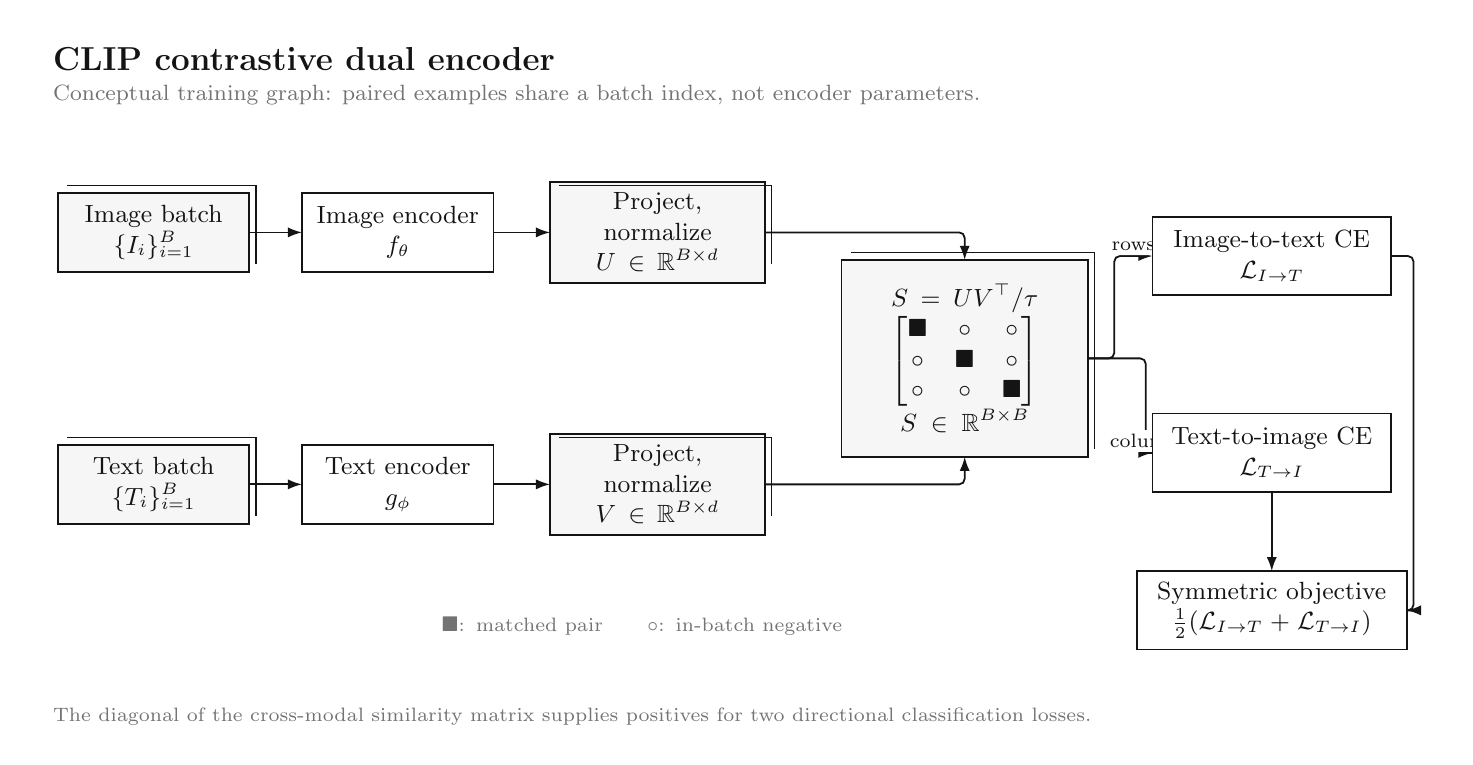
\begin{tikzpicture}[x=1cm,y=-1cm,font=\rmfamily,text=ink]

\path[use as bounding box] (0,0) rectangle (18,9);
\node[anchor=west,font=\large\bfseries] at (.2,.4) {CLIP contrastive dual encoder};
\node[anchor=west,font=\footnotesize,text=soft] at (.2,.85) {Conceptual training graph: paired examples share a batch index, not encoder parameters.};
\begin{pgfonlayer}{background}
\end{pgfonlayer}
\node[box,fill=wash,minimum width=2.4cm,minimum height=1cm,text width=2.15cm] (images) at (1.6,2.6) {Image batch\\$\{I_i\}_{i=1}^{B}$};
\draw[ink,line width=.4pt] (0.5000000000000001,2.0) -- (2.9,2.0) -- (2.9,3.0);
\node[box,fill=wash,minimum width=2.4cm,minimum height=1cm,text width=2.15cm] (texts) at (1.6,5.8) {Text batch\\$\{T_i\}_{i=1}^{B}$};
\draw[ink,line width=.4pt] (0.5000000000000001,5.2) -- (2.9,5.2) -- (2.9,6.2);
\node[box,minimum width=2.4cm,minimum height=1cm,text width=2.15cm] (vision) at (4.7,2.6) {Image encoder\\$f_{\theta}$};
\node[box,minimum width=2.4cm,minimum height=1cm,text width=2.15cm] (language) at (4.7,5.8) {Text encoder\\$g_{\phi}$};
\node[box,fill=wash,minimum width=2.7cm,minimum height=1cm,text width=2.45cm] (u) at (8.0,2.6) {Project, normalize\\$U\in\mathbb{R}^{B\times d}$};
\draw[ink,line width=.4pt] (6.75,2.0) -- (9.45,2.0) -- (9.45,3.0);
\node[box,fill=wash,minimum width=2.7cm,minimum height=1cm,text width=2.45cm] (v) at (8.0,5.8) {Project, normalize\\$V\in\mathbb{R}^{B\times d}$};
\draw[ink,line width=.4pt] (6.75,5.2) -- (9.45,5.2) -- (9.45,6.2);
\node[box,fill=wash,minimum width=3.1cm,minimum height=2.5cm,text width=2.85cm] (sim) at (11.9,4.2) {$S=UV^{\top}/\tau$\\$\begin{bmatrix}\blacksquare&\circ&\circ\\\circ&\blacksquare&\circ\\\circ&\circ&\blacksquare\end{bmatrix}$\\$S\in\mathbb{R}^{B\times B}$};
\draw[ink,line width=.4pt] (10.45,2.85) -- (13.55,2.85) -- (13.55,5.3500000000000005);
\node[box,minimum width=3.0cm,minimum height=1cm,text width=2.75cm] (row) at (15.8,2.9) {Image-to-text CE\\$\mathcal L_{I\to T}$};
\node[box,minimum width=3.0cm,minimum height=1cm,text width=2.75cm] (col) at (15.8,5.4) {Text-to-image CE\\$\mathcal L_{T\to I}$};
\node[box,minimum width=3.4cm,minimum height=0.9cm,text width=3.15cm] (loss) at (15.8,7.4) {Symmetric objective\\$\frac12(\mathcal L_{I\to T}+\mathcal L_{T\to I})$};
\begin{pgfonlayer}{background}
\draw[flow] (images.east) -- (vision.west);
\draw[flow] (texts.east) -- (language.west);
\draw[flow] (vision.east) -- (u.west);
\draw[flow] (language.east) -- (v.west);
\draw[flow] (u.east) -- (11.9,2.6) -- (sim.north);
\draw[flow] (v.east) -- (11.9,5.8) -- (sim.south);
\draw[flow] (sim.east) -- (13.8,4.2) -- (13.8,2.9) -- (row.west) node[midway,above,fill=white,inner sep=1.5pt,font=\scriptsize] {rows};
\draw[flow] (sim.east) -- (14.2,4.2) -- (14.2,5.4) -- (col.west) node[midway,above,fill=white,inner sep=1.5pt,font=\scriptsize] {columns};
\draw[flow] (row.east) -- (17.6,2.9) -- (17.6,7.4) -- (loss.east);
\draw[flow] (col.south) -- (loss.north);
\end{pgfonlayer}
\node[annotation,text width=7.0cm] at (7.8,7.6) {$\blacksquare$: matched pair\qquad $\circ$: in-batch negative};
\node[anchor=west,align=left,font=\scriptsize,text=soft,text width=17.6cm] at (.2,8.75) {The diagonal of the cross-modal similarity matrix supplies positives for two directional classification losses.};
\end{tikzpicture}
\end{document}
